\documentclass[12pt,reqno, twoside]{amsbook}
%%%%%%%%%%%%%%%%%%%%%%%%%%%%%%%%%%%%%%%%%%%%%%%%%%%%%%%%%%%%%%%%%%%%%%%%%%%%%%%%%%%%%%%%%%%%%%%%%%%%%%%%%%%%%%%%%%%%%%%%%%%%%%%%%%%%%%%%%%%%%%%%%%%%%%%%%%%%%%%%%%%%%%%%%%%%%%%%%%%%%%%%%%%%%%%%%%%%%%%%%%%%%%%%%%%%%%%%%%%%%%%%%%%%%%%%%%%%%%%%%%%%%%%%%%%%
\usepackage{eurosym}
\usepackage{amsmath}
\usepackage{amssymb}
\usepackage{amsfonts}
\usepackage[onehalfspacing]{setspace}
\usepackage{chngcntr}
\usepackage{graphicx}
\usepackage[a4paper, margin=2.5cm]{geometry}
\usepackage[english]{babel}
\usepackage{fancyhdr}
\usepackage{titlesec}
\usepackage{enumitem}
\usepackage{etoolbox}
% you may need to uncomment the command below if you use eps format for figures
%\usepackage{epstopdf}

% These packages are not part of the template made available by ISCTE
\usepackage{xcolor}
\usepackage{url}
\usepackage[printonlyused]{acronym}
\usepackage[normalem]{ulem}
\usepackage{placeins}
\usepackage{caption}
\usepackage{subcaption}
\numberwithin{figure}{chapter}
\numberwithin{table}{chapter}
%end of the extra packages


\makeatletter
    \def\section{\@startsection{section}{1}%
      \z@{.5\linespacing\@plus.7\linespacing}{.25\linespacing}%
      {\normalfont\bfseries\flushleft}}
    \def\subsection{\@startsection{subsection}{2}%
      \z@{.5\linespacing\@plus.7\linespacing}{.25\linespacing}%
      {\normalfont\bfseries\flushleft}}

\makeatother
\setcounter{MaxMatrixCols}{10}

\providecommand{\U}[1]{\protect\rule{.1in}{.1in}}
\theoremstyle{plain}
\newtheorem{acknowledgement}{Acknowledgement}
\newtheorem{algorithm}{Algorithm}[chapter]
\newtheorem{axiom}{Axiom}[chapter]
\newtheorem{case}{Case}[chapter]
\newtheorem{claim}{Claim}[chapter]
\newtheorem{conclusion}{Conclusion}[chapter]
\newtheorem{condition}{Condition}[chapter]
\newtheorem{conjecture}{Conjecture}[chapter]
\newtheorem{corollary}{Corollary}[chapter]
\newtheorem{criterion}{Criterion}[chapter]
\newtheorem{definition}{Definition}[chapter]
\newtheorem{example}{Example}[chapter]
\newtheorem{exercise}{Exercise}[chapter]
\newtheorem{lemma}{Lemma}[chapter]
\newtheorem{notation}{Notation}[chapter]
\newtheorem{problem}{Problem}[chapter]
\newtheorem{proposition}{Proposition}[chapter]
\newtheorem{remark}{Remark}[chapter]
\newtheorem{solution}{Solution}[chapter]
\newtheorem{summary}{Summary}[chapter]
\newtheorem{theorem}{Theorem}[chapter]
\numberwithin{equation}{chapter}


% Please write the references according to your school

\newenvironment{dedication}
  {%\clearpage           % we want a new page
   \thispagestyle{empty}% no header and footer
   \vspace*{\stretch{1}}% some space at the top
   \itshape             % the text is in italics
   \raggedleft          % flush to the right margin
  }
  {\par % end the paragraph
   \vspace{\stretch{3}} % space at bottom is three times that at the top
   %\clearpage           % finish off the page
  }
  \numberwithin{section}{chapter}
\fancyhead{}
\fancyfoot{}
\pagestyle{fancy}
\fancyfoot[LE,RO]{\thepage}

\makeatletter
\def\ps@plain{\ps@empty
 \def\@evenfoot{%
   \normalfont\scriptsize
   \rlap{\thepage}\hfil
   }%
 \def\@oddfoot{%
   \normalfont\scriptsize \hfil
   \llap{\thepage}}%
}
\makeatother
\renewcommand{\headrulewidth}{0pt}
\renewcommand{\footrulewidth}{0pt}






%%%%%%%%%%%%%%%%%%%%%%%%%%%%%%%%%%%%%%%%%%%%%%%%%%%%%%%%%%%%%%%%%%%%%%%%%%%%%%%%%%%%%%%%
% Cover that doesn't come with the template provided by ISCTE
% Overleaf says there are errors with this section, but it renders fine so just ignore them

\definecolor{coverline}{RGB}{66, 81, 160}
\def\hrulefill{\leavevmode\leaders\hrule height 2pt\hfill\kern\z}

\begin{document}

\sffamily
\begin{flushleft}

\includegraphics[width=6.03cm]{images/iscte}\\[3mm]
\begin{large}
{\fontfamily{Montserrat-TOsF}\selectfont
{\color{coverline} \hrulefill}
~\\
~\\
The Dissertation Title\\
~\\
~\\
The author's name\
~\\
~\\
Master's in XXXXX XXXXX\\
~\\
~\\
~\\
Supervisor:\\
PhD Ana Maria de Almeida, Associate Professor,  \\
ISCTE, Departamento de Ciências e Tecnologias de Informação\\
~\\
Co-Supervisor:\\
PhD X Y Z Name , {Full Professor, Associate Professor, Assistant Professor},\\
ISCTE, Departamento de X Y Z \\
~\\
~\\
~\\
Month, Year}
\end{large}
\end{flushleft}
\thispagestyle{empty}
\cleardoublepage
\begin{flushleft}
 % 
\includegraphics[width=6.03cm]{images/ista.png}\\[7mm]
 \begin{figure}[h]
  \centering
  \subfloat{
\includegraphics[width=.34\linewidth]{images/ista.png}}\hfill
  \subfloat {
\includegraphics[width=.34\linewidth]{images/ibs.png}}
\end{figure}
\begin{large}
{\fontfamily{Montserrat-TOsF}\selectfont
{\color{coverline} \hrulefill}
~\\
~\\
Department of Information Sciences and Technologies
~\\
Department of Quantitative Methods for Management and Economics
~\\
~\\
Dissertation Name\\
~\\
~\\
Author name\\
~\\
~\\
Master's in Data Science\\
~\\
~\\
~\\
Supervisor:\\
PhD Ana Maria de Almeida, Associate Professor,  \\
ISCTE, Departamento de Ciências e Tecnologias de Informação\\
~\\
Co-Supervisor:\\
PhD X Y Z Name , {Full Professor, Associate Professor, Assistant Professor},\\
ISCTE, Departamento de X Y Z \\
~\\
~\\
~\\
September 2025}
\end{large}
  \end{flushleft}
  \thispagestyle{empty}
\rmfamily
\normalsize
\frontmatter
\frontmatter
%\addtocontents{toc}{\setcounter{tocdepth}{2}}
\addtocontents{toc}{\setcounter{tocdepth}{2}}
\thispagestyle{empty}
\thispagestyle{empty}
\counterwithout{figure}{chapter}

\frontmatter
\addtocontents{toc}{\setcounter{tocdepth}{2}}
\thispagestyle{empty}
%%%%%%%%%%%%%%%%%%%%%%%%%%%%%%%%%%%%%%%%%%%%%%%%%%%%%%%%%%%%%%%%%%%%%%%%%%%%%%%%%%%%%%%%%%%%%%%%%%%%%%%%%%%%
\counterwithin{figure}{chapter}




%\begin{document}
\frontmatter
\addtocontents{toc}{\setcounter{tocdepth}{2}}
\thispagestyle{empty}

\begin{dedication}%

\begin{flushright}
\textit{Write here your dedication}
\end{flushright}%
\end{dedication}

\setcounter{page}{1}
\pagenumbering{roman} %
\chapter*{Acknowledgment}

Write here the acknowledgements and grants, if any

\chapter*{Resumo}

Write here your abstract in Portuguese

\chapter*{Abstract}

Write here your abstract in English


\tableofcontents

%%%%%%%%%%%%%%%%%%%%%%%%%%%%%%%%%%%%%%%%%%%%%%%%%%%%%%%%%%%%%%%%%%%%%%%%%%%%%%%%%%%%%%%%%%%%%%%%%%%%%%%%%%%%%%%%%%%
% Also not in the original template
% Remove the ones you don't need
\listoffigures

\listoftables
\cleardoublepage

\chapter*{List of Acronyms}
% Acronyms -- Optional, but you should use them if you use acronyms in your text!
%
% You can define as many acronyms as you want, like this:
%   \acro{TIAA}{This Is An Acronym}
% IN ALPHABETICAL ORDER
% You can reference an acronym as-is inline using e.g. \ac{TIAA}.
% If you need to reference a pluralised acronym, instead use \acp.
    \begin{acronym}
        \acro{AI}{Artificial Intelligence}
        \acro{COV}{COVID-19}
        \acro{DSR}{Design Science Research}
        \acro{IS}{Information System}
    \end{acronym}


\cleardoublepage
%\printglossary[type=\acronymtype, nonumberlist, nogroupskip]

%%%%%%%%%%%%%%%%%%%%%%%%%%%%%%%%%%%%%%%%%%%%%%%%%%%%%%%%%%%%%%%%%%%%%%%%%%%%%%%%%%%%%%%%%%%%%%%%%%%%%%%%%%%%%%%%%%



\mainmatter



\hyphenation{wri-te he-re pro-per hy-phe-ni-za-tion}%

\setcounter{page}{1} \pagenumbering{arabic}



% =====================================================================
%                               MAIN BODY
% =====================================================================
\begin{document}


%%%%%%%%%%%%%%%%%%%%%%%%%%%%%%%%%%%%%%%%%%%%%%%%%%%%%%%%
\chapter{Introduction}
\label{chapter:intro}
%%%%%%%%%%%%%%%%%%%%%%%%%%%%%%%%%%%%%%%%%%%%%%%%%%%%%%%
%\noindent You must use $\backslash$noindent at the beginning of the first paragraph in sections and subsections.

%%%%%%%%%%%%%%%%%%%%%%%
%%%%%%%%%%%%%%%%%%%%%%%
\section{Context}
\label{section:context}
\noindent  The global pandemic triggered in 2019 by the \ac{COV} and declared by the World Health Organization on March 11, 2020 \cite{who-covid19}, has exposed inherent weaknesses in health systems worldwide.


This dissertation aims to contribute to the development of a mobile health application enahnaced by an \ac{AI}  in a project coordinated by the Center for Research in Science, Technology and Architecture (ISTAR-Iscte), under grant number XYZ.\par

%%%%%%%%%%%%%%%%%%%%%%%
%%%%%%%%%%%%%%%%%%%%%%%
\section{Motivation} 
\label{section:motivation}
\noindent This research is motivated by altruistic aims. \par


\par

\section{Problem} 
\noindent The central challenge lies in the scarcity of advanced mHealth applications capable of efficiently collecting health data, performing continuous monitoring, accurate diagnosis, and offering personalized health services, all while guaranteeing the privacy and security of user data.  \par


\vspace{\baselineskip}


%%%%%%%%%%%%%%%%%%%%%%%
%%%%%%%%%%%%%%%%%%%%%%%
\section{Objectives and Research Questions} 
\label{section:objectives}
\noindent  Considering the challenges presented in the research,

\begin{enumerate}[leftmargin=1.5cm,label=RQ\arabic*:,itemsep=.5ex]
                 \item …
                 \item …
\end{enumerate}

%%%%%%%%%%%%%%%%%%%%%%%
%%%%%%%%%%%%%%%%%%%%%%%
\section{Methodology} 
\label{section:objectives}

Our methodology is based on \ac{DSR} to attain its goals and answer the research questions.



%We add a page brake to show that the even page number appears on the left
\newpage

%%%%%%%%%%%%%%%%%%%%%%%%%%%%%%%%%%%%%%%%%%%%%%%%%%%%%%%%
\chapter{Literature Review}
\label{chapter:LitReview}
%%%%%%%%%%%%%%%%%%%%%%%%%%%%%%%%%%%%%%%%%%%%%%%%%%%%%%%%
\noindent  This section will look at Federated Learning techniques and data processing in mobile health (mHealth), exploring the application of machine learning methods and real-time signal processing for analyzing medical data. Techniques aimed at the early detection of anomalous patterns, such as changes in heart rhythms, which can indicate potential health problems in users in mHealth environments, will be discussed. \par

%%%%%%%%%%%%%%%%%%%%%%%
%%%%%%%%%%%%%%%%%%%%%%%
\section{Systematic Literature Review }
\label{section:SLR}

\noindent Following the \ac{PRISMA} methodology\footnote{PRISMA: \url{http://www.prisma-statement.org/}}, the search for papers related to the dissertation had to be carried out in several repositories. The repositories used were the IEEE Xplore Digital Library\footnote{IEEE Xplore: \url{https://ieeexplore.ieee.org/Xplore/home.jsp}}, Web of Science database\footnote{Web of Science: \url{https://www.webofscience.com/wos/woscc/basic-search}} and Scopus database\footnote{Scopus: \url{https://www.scopus.com/search/form.uri?display=basic#basic}}. 

%%%%%%%%%%%%%%%%%%%%%%%
%%%%%%%%%%%%%%%%%%%%%%%
\section{Discussion of Related Work} 
\label{section:relatedwork}

\noindent In recent years, there has been a significant increase in the number of articles exploring how  


%%%%%%%%%%%%%%%%%%%%%%%
\subsection{Federated Learning in XYZ} 
\label{subsection:FLXYZ}

\noindent The literature review highlights \subsection{Federated Learning in Cardiovascular and Neurological Health} 

\noindent An analysis of studies focusing on the use of Federated Learning in cardiovascular and neurological health reveals significant advances. 


%%%%%%%%%%%%%%%%%%%%%%%
\subsection{Federated Learning and COVID-19}
\label{subsection:FLC}

\noindent The literature has explored various strategies to address the COVID-19 pandemic through Federated Learning, resulting in a wide variety of articles dedicated to this topic. 

%%%%%%%%%%%%%%%%%%%%%%%
\subsection{Summary}
\label{subsection:summary}

\noindent Although there are several mobile healthcare applications that employ .




%%%%%%%%%%%%%%%%%%%%%%%%%%%%%%%%%%%%%%%%%%%%%%%%%%%%%%%%
\chapter{Methodology}
\label{chapter:Methodology}

...
%%%%%%%%%%%%%%%%%%%%%%%%%%%%%%%%%%%%%%%%%%%%%%%%%%%%%%%%




%%%%%%%%%%%%%%%%%%%%%%%%%%%%%%%%%%%%%%%%%%%%%%%%%%%%%%%%
\chapter{Results}
\label{chapter:ExpRes}

...
%%%%%%%%%%%%%%%%%%%%%%%%%%%%%%%%%%%%%%%%%%%%%%%%%%%%%%%%




%%%%%%%%%%%%%%%%%%%%%%%%%%%%%%%%%%%%%%%%%%%%%%%%%%%%%%%%%%%%%%%%%%%%%%%%%%%%%%%%%%%%%%%%%%
\chapter{Added Things: some extra things that might be helpful}
\noindent This chapter isn't in the template provided by ISCTE and contains some extra things that might be helpful.


\section{Glossary}
This section explains how to use a package that handles the abbreviations. Near line 107 there's the following code:
\begin{verbatim}
    \DeclareAcronym{wip}{
        short=WIP,
        long=work in progress,
    }
\end{verbatim}

Be WIP an acronym for "work in progress" and "wip", the first time $\backslash$ac\{wip\} is written, the package writes \ac{wip}. The next time it's used, it only writes \ac{wip}.

Pay attention to acronyms with very long meanings as the package does not handle them well.

\section{Lists}
An example of a bullet list
\begin{itemize}
    \item Potatoes
    \item Lettuce
\end{itemize}

An example of an ordered list
\begin{enumerate}
    \item A
    \item B
    \item C
\end{enumerate}

\section{Bibliography}
\noindent To reference the bibliography, write the bib of the reference in the references.bib file then use $\backslash$cite\{\}. Example: \cite{firouzi2021}. The bibliography is already getting added and numbered according to when they are referenced.

%%%%%%%%%%%%%%%%%%%%%%%%%%%%%%%%%%%%%%%%%%%%%%%%%%%%%%%%%%%%%%%%%%%%%%%%%%%%%%%%%%%%%%%%%%%%%%

\section{Tables}
\noindent Check the code on this section to see how to make a table. 
Both tables and images might not appear where you expect them to appear to save up space.

\begin{table}
    \centering
    \begin{tabular}{c|cc}
        A & B & C\\
        \hline
        1 & 2 & 3\\
        a & b & c\\
        0 & \multicolumn{2}{|c|}{99}
    \end{tabular}
    \caption{Caption}
    \label{a_table}
\end{table}

%%%%%%%%%%%%%%%%%%%%%%%%%%%%%%%%%%%%%%%%%%%%%%%%%%%%%%%%%%%%%%%%%%%%%%%%%%%%%%%%%%%%%%%%%%%%%

\section{Images}
\noindent Here are two examples of how to place images in the document.
\begin{figure}[h!]
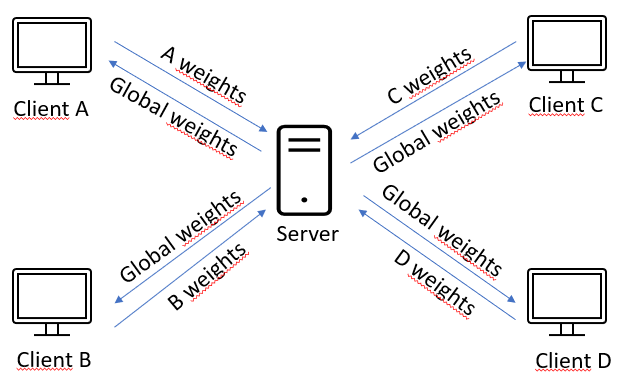
\includegraphics[width=\textwidth]{images/fl.png}
\caption{An example of a picture} \label{fig_example1}
\end{figure}

\begin{figure}
     \centering
     \begin{subfigure}[b]{0.45\textwidth}
         \centering
         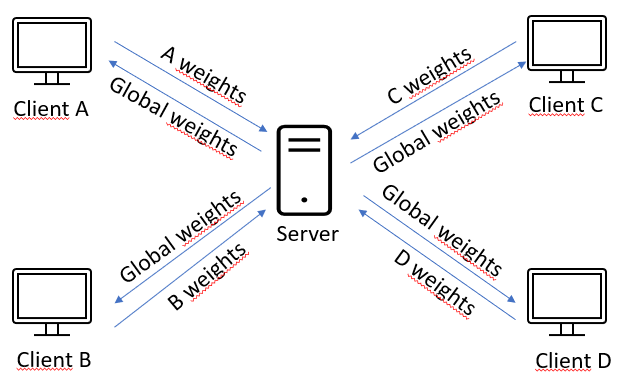
\includegraphics[width=\textwidth]{images/fl.png}
         \caption{Figure on the left}
         \label{fig_example2a}
     \end{subfigure}
     \hfill
     \begin{subfigure}[b]{0.45\textwidth}
         \centering
         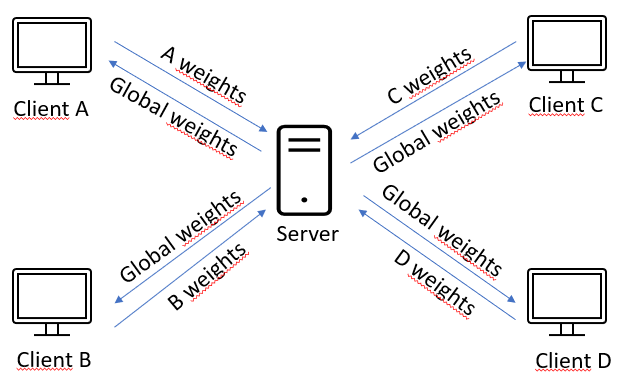
\includegraphics[width=\textwidth]{images/fl.png}
         \caption{Figure on the right}
         \label{fig_example2b}
     \end{subfigure}
        \caption{I reused the same picture}
        \label{fig_example2}
\end{figure}



%%%%%%%%%%%%%%%%%%%%%%%%%%%%%%%%%%%%%%%%%%%%%%%%%%%%%%%%%%%%%%%%%%%%%%%%%%%%%%%%%%%%%%%%%%%


%%%%%%%%%%%%%%%%%%%%%%%%%%%%%%%%%%%%%%%%%%%%%%%%%%%%%%%%
\chapter{Conclusions}
\label{chapter:Conclusion}
%%%%%%%%%%%%%%%%%%%%%%%%%%%%%%%%%%%%%%%%%%%%%%%%%%%%%%%%




\renewcommand{\bibname}{References}

%%%%%%%%%% ADDED %%%%%%%%%%%%
\bibliographystyle{IEEEtran}
\bibliography{references}
%%%%%%%%%%%%%%%%%%%%%%%%%%%%%%

\appendix
\chapter{} \label{appendixA}
\noindent An appendix

\end{document}
